
%(BEGIN_QUESTION)
% Copyright 2012, Tony R. Kuphaldt, released under the Creative Commons Attribution License (v 1.0)
% This means you may do almost anything with this work of mine, so long as you give me proper credit

Suppose you are asked to do a ``trip test'' of the high-temperature shutdown controls for this natural gas compressor system.  You need to test both the motor's high-temperature shutdown function as well as the compressor's high-temperature shutdown function.  Your test(s) need to be a thorough and realistic as possible, but without actually interrupting the compression of natural gas!

$$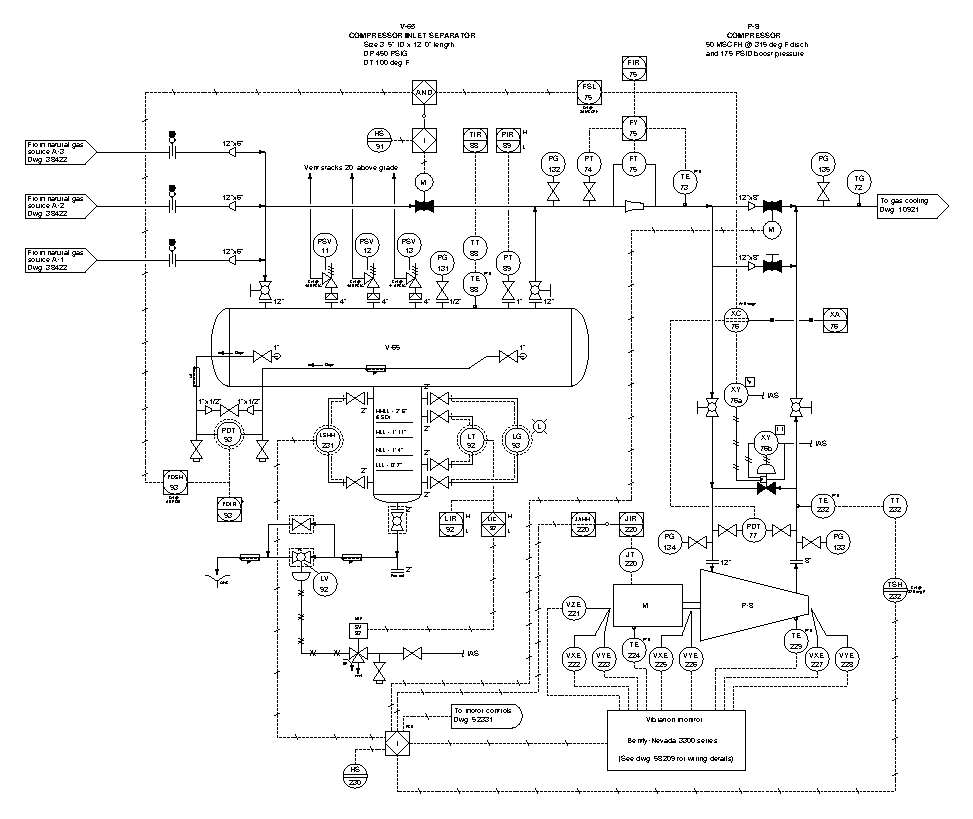
\includegraphics[width=15.5cm]{i0003rx01.eps}$$

Explain how you would simulate a high-temperature condition, and also how you would verify the proper operation of the emergency shutdown system (ESD) while ensuring the compressor does not actually shut down.

\vskip 20pt \vbox{\hrule \hbox{\strut \vrule{} {\bf Suggestions for Socratic discussion} \vrule} \hrule}

\begin{itemize}
\item{} Based on what you see in this diagram, explain the purpose of the emergency shutdown system.  What conditions, specifically, is it looking for to trip, and what are the consequences of a trip?
\end{itemize}

\underbar{file i01242}
%(END_QUESTION)





%(BEGIN_ANSWER)

Simulation hint: the temperature sensors are {\it RTDs}.

%(END_ANSWER)





%(BEGIN_NOTES)

Connecting a potentiometer in place of the RTD would allow you to simulate any temperature condition desired.  In order to avoid tripping this compressor system, you would have to disable/disconnect the bypass valve as well as any motor controls represented on drawing 52331.  Then, you would use a meter to ensure the presence of the correct ``trip'' signals to those disabled final control elements during your test.




\vskip 20pt \vbox{\hrule \hbox{\strut \vrule{} {\bf Virtual Troubleshooting} \vrule} \hrule}

This question is a good candidate for a ``Virtual Troubleshooting'' exercise.  Presenting the diagram to students, you first imagine in your own mind a particular fault in the system.  Then, you present one or more symptoms of that fault (something noticeable by an operator or other user of the system).  Students then propose various diagnostic tests to perform on this system to identify the nature and location of the fault, as though they were technicians trying to troubleshoot the problem.  Your job is to tell them what the result(s) would be for each of the proposed diagnostic tests, documenting those results where all the students can see.

During and after the exercise, it is good to ask students follow-up questions such as:

\begin{itemize}
\item{} What does the result of the last diagnostic test tell you about the fault?
\item{} Suppose the results of the last diagnostic test were different.  What then would that result tell you about the fault?
\item{} Is the last diagnostic test the best one we could do?
\item{} What would be the ideal order of tests, to diagnose the problem in as few steps as possible?
\end{itemize}

\vskip 20pt \vbox{\hrule \hbox{\strut \vrule{} {\bf Virtual Trip-testing} \vrule} \hrule}

This question is a good candidate for a ``Virtual Trip-testing'' exercise.  Presenting the diagram to students, you pose an assignment whereby students must figure out how to test some component of this system to check that it will operate as intended to shut down the system in an abnormal (trip) condition, with some realistic limitation (e.g. power cannot be shut off to the load).  Students then propose various methods for executing the test.  Your job is to determine whether or not their proposed tests will achieve the desired result(s).

During and after the exercise, it is good to ask students follow-up questions such as:

\begin{itemize}
\item{} Where might our planned test strategy go wrong?  In other words, what thing(s) might happen to foil our test, either to invalidate the results or to not honor the stated limitation(s)?
\item{} Suppose the limitation were different.  How would this affect our ability to carry out the test?
\item{} Is the last test strategy best one we could execute?
\end{itemize}


%INDEX% Process: gas compressor inlet separator (realistic P&ID shown)
%INDEX% Safety, shutdown system: trip testing

%(END_NOTES)

